\begin{frame}
\frametitle{Etapa 1: Cliques Maximales}
	
%\begin{itemize}
%	\item Es un problema complejo desde un punto de vista teórico y práctico. 
%	\item \textit{Eppstein, Strash et. al.} proponen un algoritmo\footnote{https://github.com/darrenstrash/quick-cliques} rápido para listar cliques maximales de grafos dispersos.
%	\item Se asume que algoritmo puede entregar el listado de cliques maximales de un grafo.
%	\item Problema a resolver: Encontrar un método eficiente para dividir en particiones el grafo de cliques.
%\end{itemize}

Es un problema complejo desde un punto de vista teórico y práctico. 

\textit{Eppstein, Strash et. al.} proponen un algoritmo\footnote{https://github.com/darrenstrash/quick-cliques} rápido para listar cliques maximales de grafos dispersos.

Se asume que algoritmo puede entregar el listado de cliques maximales de un grafo.

Problema a resolver: Encontrar un método eficiente para dividir en particiones el grafo de cliques.

\end{frame}


\begin{frame}
\frametitle{Etapa 1: Cliques Maximales (2)}

\begin{definition} 
	\label{def:cliqueGraph}
	Gafo de cliques
	
	Dado un grafo $G = (V, E)$ y $\mathcal{C} = \{c_{1}, c_{2}, ..., c_{N} \}$ el conjunto de tamaño $N$ de cliques maximales que cubren $G$, se tiene $CG_{\mathcal{C}} = (V_{\mathcal{C}}, E_{\mathcal{C}})$ un grafo de cliques donde:
	
	\begin{enumerate}
		\item $V_{\mathcal{C}} = \mathcal{C}$
		\item $\forall c, c' \in \mathcal{C}, (c, c') \in E_{\mathcal{C}} \Longleftrightarrow c \cap c' \neq \varnothing$
	\end{enumerate}
\end{definition}

\end{frame}


\begin{frame}
\frametitle{Etapa 1: Cliques Maximales (3)}

\begin{figure}
    	\centering
    	\begin{minipage}{0.45\textwidth}
    		\centering
    		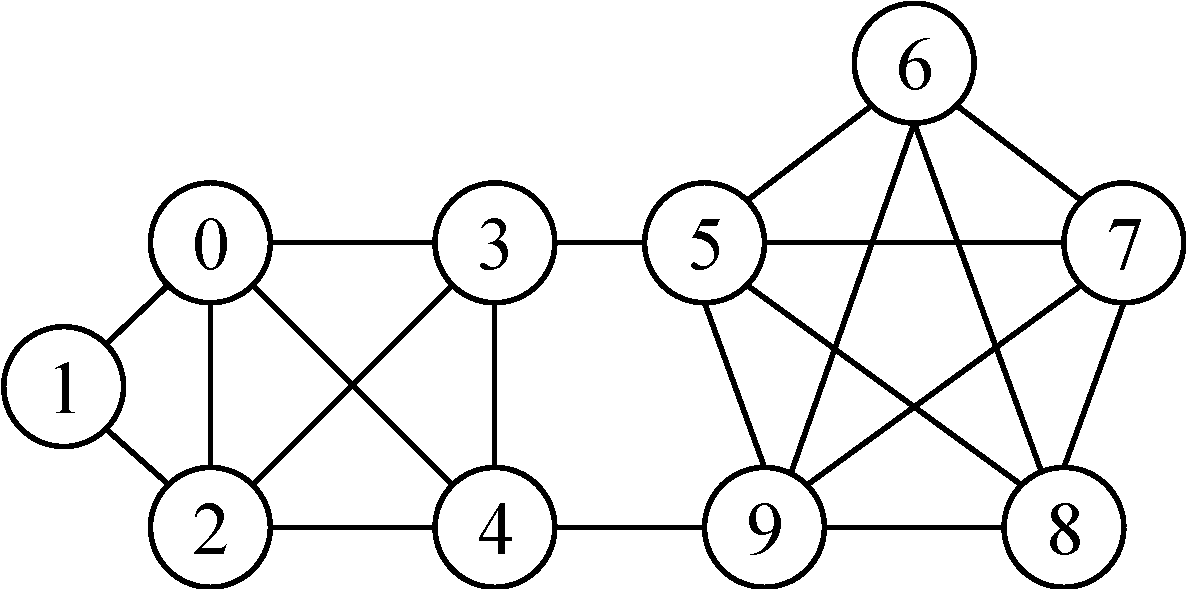
\includegraphics[width=1\linewidth,clip=true]{../img/graphs-Graph2.pdf}
    		(a)
    	\end{minipage}
    	\begin{minipage}{0.25\textwidth}
    		\centering
    		\[
	\begin{aligned}[t]
		C_{0} &: 0, 1, 2 \\
		C_{1} &: 0, 2, 3, 4 \\
		C_{2} &: 3, 5 \\
		C_{3} &: 5, 6, 7, 8, 9 \\
		C_{4} &: 4, 9
	\end{aligned}
\]

    		(b)
    	\end{minipage}
    	\begin{minipage}{0.15\textwidth}
    		\centering
    		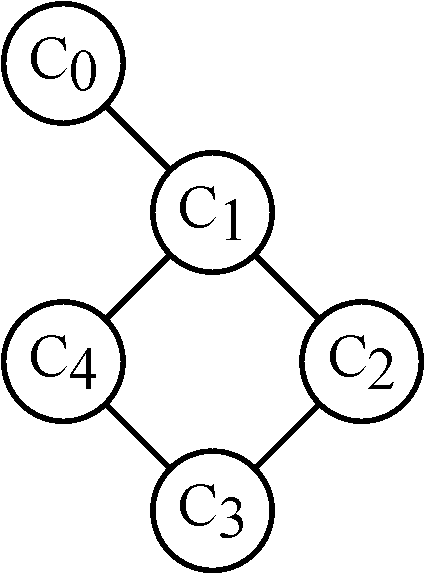
\includegraphics[width=1\linewidth,clip=true]{../img/graphs-Cliques2.pdf}
    		(c)
    	\end{minipage}
    \caption{(a) Grafo no dirigido. (b) Lista de cliques maximales. (c) Grafo de cliques.}
    \label{fig:gafoEj}
\end{figure}

\end{frame}
